% \chapter{Intrinsic experiments}
% \label{cha:experiments}

% Table~\ref{tab:parameters} lists parameters and their values. As the source corpus we use the concatenation of Wackypedia and ukWaC \cite{ukwac} with a symmetric 5-word window \cite{milajevs-EtAl:2014:EMNLP2014}; the evaluation metric is the correlation with human judgements as is standard with SimLex \cite{hill2014simlex} and other lexical datasets.

% We derive our parameter selection heuristics by greedily selecting parameters (\texttt{cds}, \texttt{neg}) that lead to the highest average performance for each combination of frequency weighting, PMI variant and dimensionality $D$. Figures~\ref{fig:interaction-cds} and \ref{fig:interaction-neg} show the interaction of \texttt{cds} and \texttt{neg} with other parameters. We also vary the similarity measure (cosine and correlation  \cite{kiela-clark:2014:CVSC}), but do not report results here due to space limits.

\chapter{Relationships between words}
\label{sec:lexical}

This chapter is dedicated to the lexical experiments. Two datasets are used: SimLex-999 \cite{hill2014simlex} and MEN \cite{Bruni:2014:MDS:2655713.2655714}. First, some of the  hypotheses in Section~\ref{sec:hypotheses} are defined more exactly. After the results and parameter selection are reported on the datasets individually, the model selection is performed on a combination of the two datasets. The models are evaluated by computing the Spearman's-$\rho$ (the correlation of ranked model predictions with ranked human judgements) as it is normally done \cite{Bruni:2014:MDS:2655713.2655714,hill2014simlex}. The results are available at \url{\BASEURL/results_all.csv}.

\section{Specialised hypotheses}
\label{sec:elab-hypoth-lexical}

Before reporting the results of the lexical experiments, we would like to expand on the hypotheses stated in Section~\ref{sec:hypotheses} to the lexical case.

\begin{hyp}[H\ref{hyp:lex-pmi-cpmi}]
  \label{hyp:lex-pmi-cpmi}
  In lexical tasks, there should be no difference between PMI and its compressed version CPMI (Section~\ref{sec:pmi-variants}).
% Shifted PMI variants behave the same (Section~\ref{sec:shifted-pmi}).
\end{hyp}

The main effect of CPMI is to transform negative values into the positive range of $(0; 1)$. The reason to avoid negative values is that they might be problematic for multiplication during composition as the sign of the result depends on the number of negative components. However as there is no composition involved in lexical tasks, the weighting schemes should behave equally.

The next hypotheses are related to PMI's Achilles heel and are supposed to lower the influence of low co-occurrence counts, therefore we expect that they are beneficial for highly dimensional spaces as partially showed in \newcite{milajevs-sadrzadeh-purver:2016:ACL-SRW}.

\begin{hyp}[H\ref{hyp:freq}]
  \label{hyp:freq}
 $N$ or $\log n$ frequency components (Section~\ref{sec:frequency-weighting}) should be beneficial for highly-dimensional spaces.
\end{hyp}

This is the most direct way of boosting high co-occurrence counts \cite{Evert05}. \NPMI/ is shown to be a good choice in lexical tasks \cite{Bruni:2012:DST:2390524.2390544}.

\begin{hyp}[H\ref{hyp:cds}]
  \label{hyp:cds}
  Low-dimensional spaces should not need context distribution smoothing, while highly-dimensional spaces should benefit from it (Section~\ref{sec:cont-distr-smooth}).
\end{hyp}

This is because the estimated probabilities of rare contexts are noisy. This smoothing is shown successful in high-dimensional count-based models \cite{TACL570} and word2vec \cite{mikolov2013efficient}. However, \newcite{milajevs-sadrzadeh-purver:2016:ACL-SRW} showed that for low-dimensional spaces benefit from global context probabilities.

\begin{hyp}[H\ref{hyp:neg}]
  \label{hyp:neg}
  Low-dimensional spaces benefit from being dense, while highly-dimensional spaces benefit from being sparse.
\end{hyp}

Sparsity is controlled by the shifting parameter $k$ (Section~\ref{sec:shifted-pmi}), lower $k$ values make vectors denser.

\section{SimLex-999}
\label{sec:simlex-999}

\subsection{Max selection}
\label{sec:max-selection-simlex}

\begin{wrapfigure}[7]{O}{0.5\textwidth}
  \vspace{-30pt}
  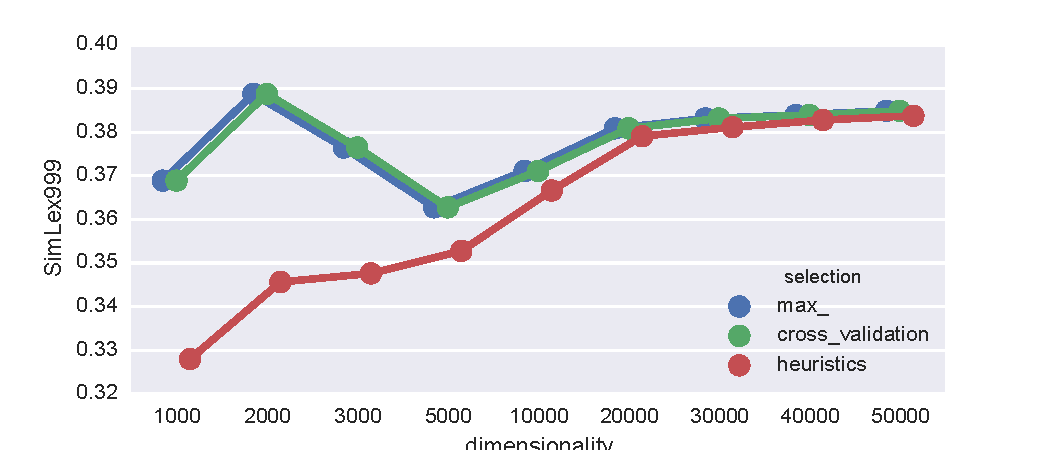
\includegraphics[width=0.5\textwidth]{supplement/figures/SimLex999-results}
  \caption{SimLex-999 results.}
  \label{fig:SimLex999-results}
\end{wrapfigure}

%%% Local Variables:
%%% mode: latex
%%% TeX-master: "../thesis"
%%% End:


Figure~\ref{fig:SimLex999-results} illustrates the results based on the best model selection and Table~\ref{tab:Simlex999-max-selection} shows the results together with picked parameters. Note that the maximum selection is identical with cross-validation: they pick the same models.

In general, model performance increases as the dimensionality increases. However, the best result of 0.389 is achieved with a 2000 dimensional space, this could, however, be an example of overfitting. Model performance becomes stable for dimensions greater than 20000.

For spaces with dimensionality less than 5000 \texttt{freq} 1 and inner product yield best results. Otherwise, cosine with \logNSCPMI/, smoothing $\alpha=0.75$ and shifting $k=0.7$ gives the best results. This supports our hypotheses H\ref{hyp:freq}, H\ref{hyp:cds} and H\ref{hyp:neg}.

\begin{table}
  \centering

  \begin{tabular}{rrlllrl}
\toprule
 dimensionality &  SimLex999 &  freq &  discr &     cds &  neg &     similarity \\
\midrule
           1\,000 &      0.369 &     1 &   spmi &       1 &  0.2 &  inner\_product \\
           2\,000 &      0.389 &     1 &  scpmi &  global &  0.7 &  inner\_product \\
           3\,000 &      0.376 &     1 &   spmi &    0.75 &  0.2 &  inner\_product \\
           5\,000 &      0.363 &  logn &  scpmi &  global &  1.0 &            cos \\
          10\,000 &      0.371 &  logn &  scpmi &       1 &  0.7 &            cos \\
          20\,000 &      0.381 &  logn &  scpmi &    0.75 &  0.7 &            cos \\
          30\,000 &      0.383 &  logn &  scpmi &    0.75 &  0.7 &            cos \\
          40\,000 &      0.384 &  logn &  scpmi &    0.75 &  0.7 &            cos \\
          50\,000 &      0.385 &  logn &  scpmi &    0.75 &  0.7 &            cos \\
\bottomrule
\end{tabular}


  \caption{SimLex-999 Max selection.}
  \label{tab:Simlex999-max-selection}
\end{table}


\subsection{Heuristics}
\label{sec:heuristics-simlex}

\begin{wraptable}[8]{O}{0.5\textwidth}
  \vspace{-1em}
  \centering

  \begin{tabular}{lr}
\toprule
      parameter &  partial $R^2$ \\
\midrule
     similarity &       0.38 \\
           freq &       0.27 \\
            neg &       0.24 \\
 dimensionality &       0.08 \\
          discr &       0.08 \\
            cds &       0.06 \\
\bottomrule
\end{tabular}


  \caption{SimLex-999 feature ablation}
  \label{tab:SimLex999-ablation}
\end{wraptable}


% \begin{figure}

  \centering

  \begin{subfigure}[t]{0.49\textwidth}
    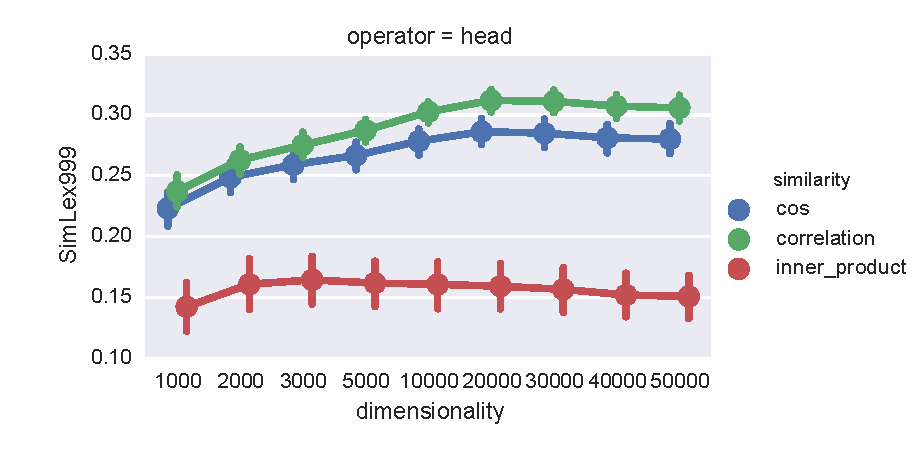
\includegraphics[width=\textwidth]{supplement/figures/SimLex999-interaction-similarity}
    \caption{similarity}
    \label{fig:SimLex999-interaction-similarity}
  \end{subfigure}
  \begin{subfigure}[t]{0.49\textwidth}
    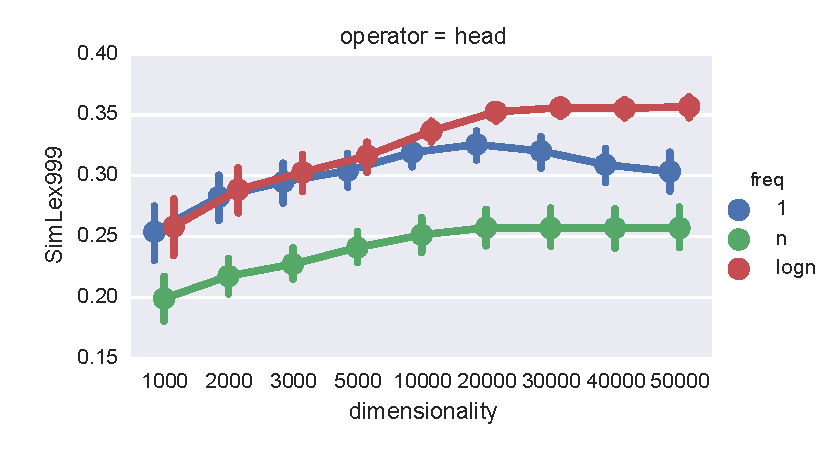
\includegraphics[width=\textwidth]{supplement/figures/SimLex999-interaction-freq}
    \caption{\texttt{freq}}
    \label{fig:SimLex999-interaction-freq}
  \end{subfigure}

  \begin{subfigure}[t]{0.49\textwidth}
    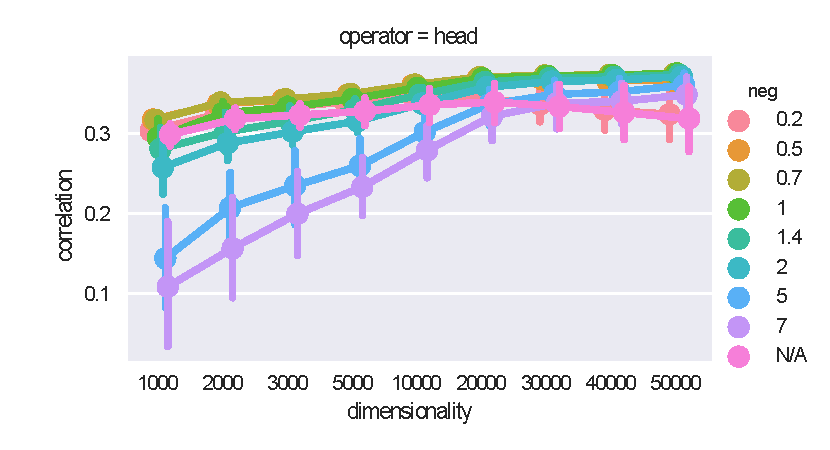
\includegraphics[width=\textwidth]{supplement/figures/SimLex999-interaction-neg}
    \caption{\texttt{neg}}
    \label{fig:SimLex999-interaction-neg}
  \end{subfigure}
  \begin{subfigure}[t]{0.49\textwidth}
    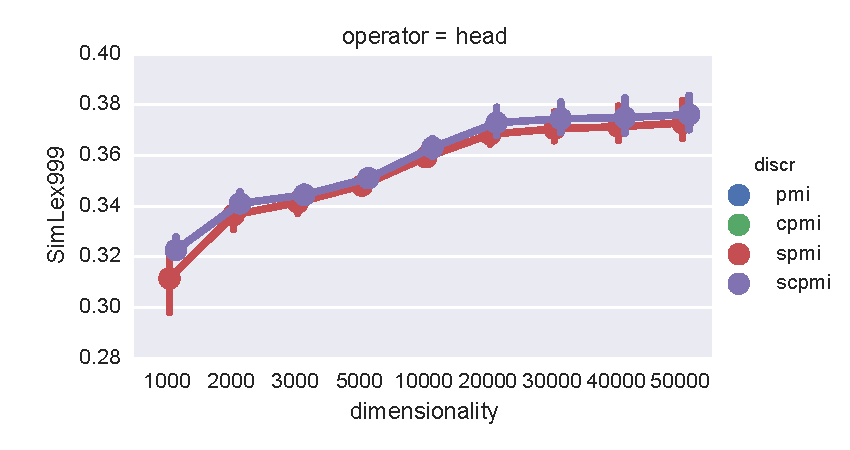
\includegraphics[width=\textwidth]{supplement/figures/SimLex999-interaction-discr}
    \caption{\texttt{discr}}
    \label{fig:SimLex999-interaction-discr}
  \end{subfigure}

  \begin{subfigure}[t]{0.49\textwidth}
    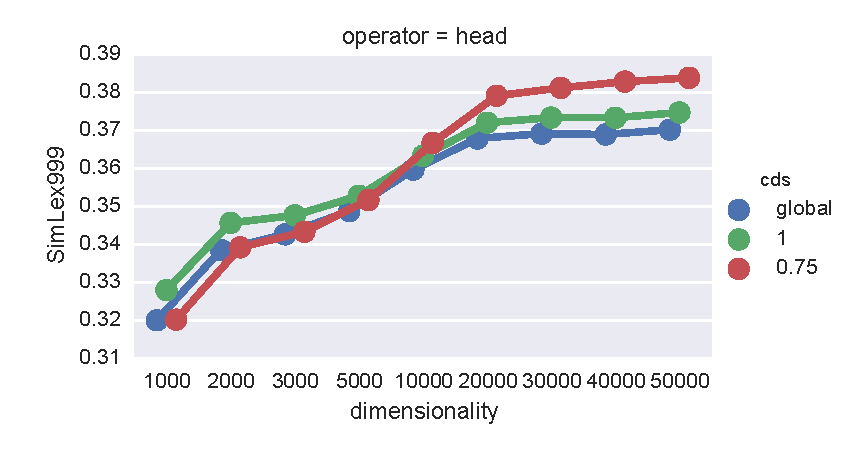
\includegraphics[width=\textwidth]{supplement/figures/SimLex999-interaction-cds}
    \caption{\texttt{cds}}
    \label{fig:SimLex999-interaction-cds}
  \end{subfigure}

  \caption{SimLex-999 parameter interaction. Parameters are shown in the order of their influence.}
  \label{fig:SimLex999-interaction}
\end{figure}

%%% Local Variables:
%%% mode: latex
%%% TeX-master: "../thesis"
%%% End:


The linear model achieves an adjusted $R^2$ of 0.867, indicating that the model is able to predict model performance based on parameter selection quite well. Table~\ref{tab:SimLex999-ablation} shows partial $R^2$ scores for parameters. The most influential parameters in decreasing order are similarity, \texttt{freq} and \texttt{neg}.

% \begin{wrapfigure}{O}{0.5\textwidth}
\begin{figure}
  % \vspace{-30pt}
  \centering

  \begin{subfigure}[t]{0.49\textwidth}
    \hspace{-20pt}
  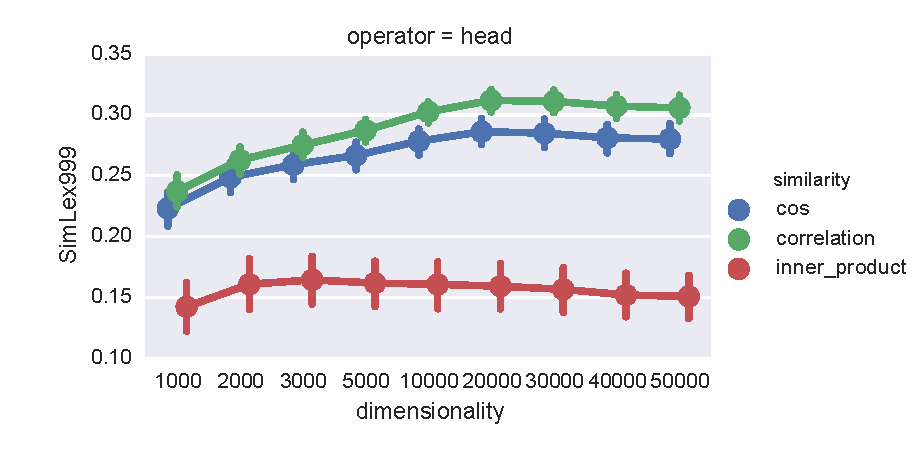
\includegraphics[width=1.1\textwidth]{supplement/figures/SimLex999-interaction-similarity}

  \caption{Similarity measure}
  \label{fig:SimLex999-similarity}

  \end{subfigure}
  \begin{subfigure}[t]{0.49\textwidth}

  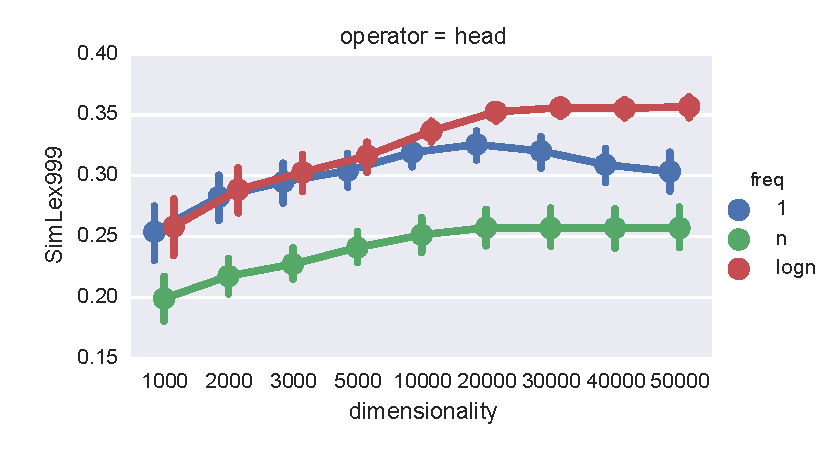
\includegraphics[width=\textwidth]{supplement/figures/SimLex999-interaction-freq}

  \caption{\texttt{freq}}
  \label{fig:SimLex999-freq}

  \end{subfigure}


  \begin{subfigure}[t]{0.49\textwidth}
  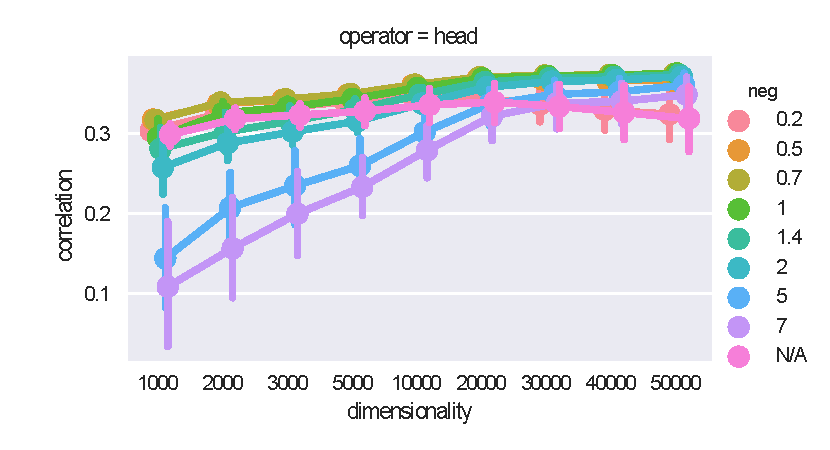
\includegraphics[width=\textwidth]{supplement/figures/SimLex999-interaction-neg}

  \caption{\texttt{neg}}
  \label{fig:SimLex999-neg}
  \end{subfigure}
  \begin{subfigure}[t]{0.49\textwidth}
  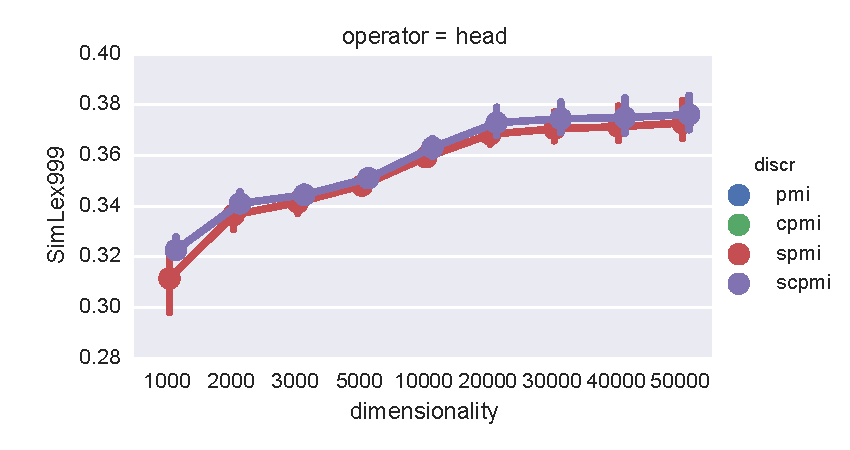
\includegraphics[width=\textwidth]{supplement/figures/SimLex999-interaction-discr}

  \caption{\texttt{discr}}
  \label{fig:SimLex999-discr}
  \end{subfigure}
  
  \caption[SimLex-999 influence of the similarity measure, \texttt{freq}, \texttt{neg} and \texttt{discr}]{SimLex-999 influence of the similarity measure, \texttt{freq}, \texttt{neg} and \texttt{discr}. Error bars indicate the 95\% confidence interval over the group of results.}
\end{figure}

Figure~\ref{fig:SimLex999-similarity} shows the average performance of similarity measures. Correlation outperforms all other measures for all dimensions and peaks at the dimensionality  of 20000 after correlation is chosen as the similarity measure. However, for $D \leq 5000$ the difference between correlation-based and cosine-based similarity measures is less than for $D > 5000$.

The influence of \texttt{freq}, the second parameter, is shown on Figure~\ref{fig:SimLex999-freq}. $\log n$ frequency outperforms other choices for all dimensions. After 20000 dimensions $\log n$'s performance stabilises: variance decreases and the performance stays constant. Taking into account that for $D \leq 5000$ there is little difference between $1$ and $\log n$, H\ref{hyp:freq} is supported in this case as well.

\begin{figure}[b]
% \begin{wrapfigure}{O}{0.5\textwidth}
  % \vspace{-30pt}
  \centering

  \begin{subfigure}[t]{0.49\textwidth}
  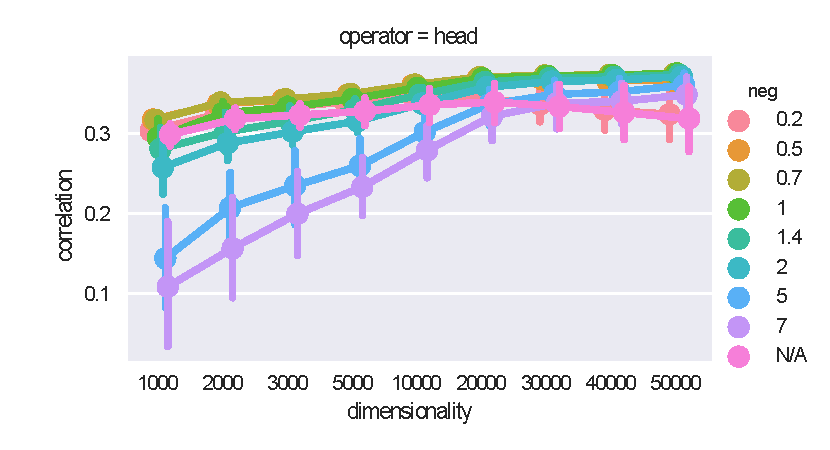
\includegraphics[width=\textwidth]{supplement/figures/SimLex999-interaction-neg}

  \caption{\texttt{neg}}
  \label{fig:SimLex999-neg}
  \end{subfigure}
  \begin{subfigure}[t]{0.49\textwidth}
  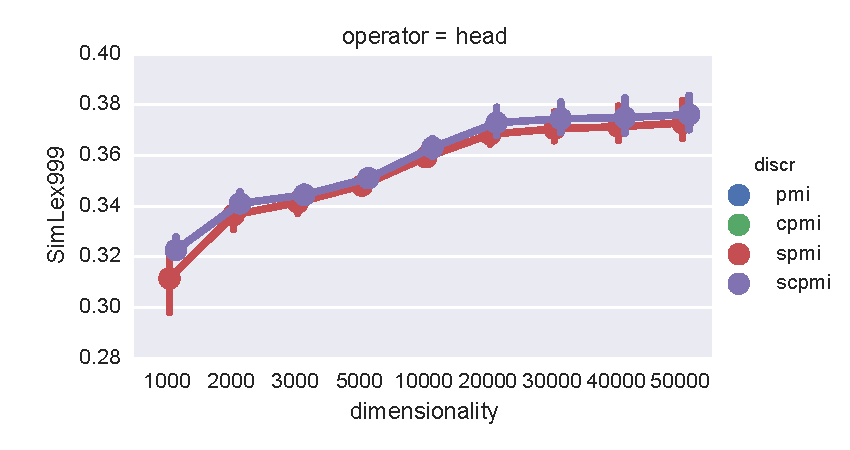
\includegraphics[width=\textwidth]{supplement/figures/SimLex999-interaction-discr}

  \caption{\texttt{discr}}
  \label{fig:SimLex999-discr}
  \end{subfigure}

  \caption{SimLex-999.}
\end{figure}

The third parameter \texttt{neg} of 0.7 shows the best performance (Figure~\ref{fig:SimLex999-neg}). However, there is little difference between models with dimensionality greater than 20000 (supporting H\ref{hyp:var} and H\ref{hyp:neg}), apart from the models that do not perform shifting, whose performance peaks at 20000 dimensions and decreases afterwards with increasing variance.

% \begin{figure}[h]
% \begin{wrapfigure}{O}{0.5\textwidth}
  % \vspace{-30pt}
  \centering

  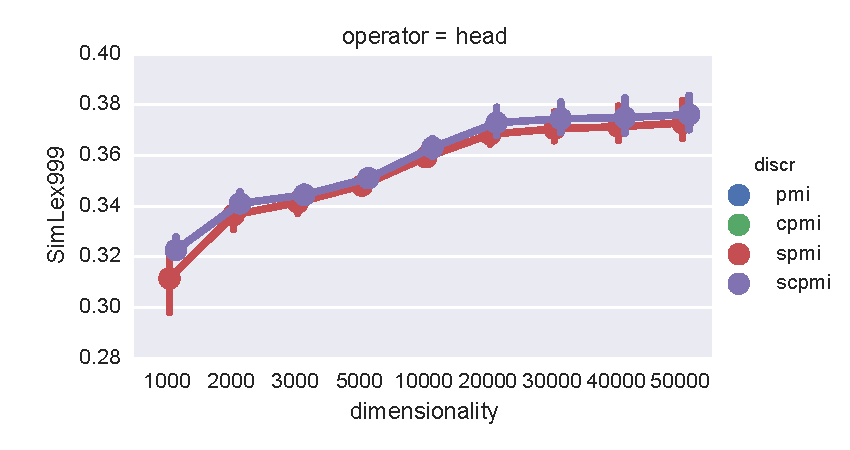
\includegraphics[width=0.5\textwidth]{supplement/figures/SimLex999-interaction-discr}

  \caption{SimLex-999 influence of \texttt{discr}. PMI and CPMI are not shown because at the step before models with shifting were chosen.}
  \label{fig:SimLex999-discr}
\end{figure}

There is little difference between SPMI and SCPMI performance with a little advantage to SCPMI (Figure~\ref{fig:SimLex999-discr}), supporting H\ref{hyp:lex-pmi-cpmi}.

% \begin{figure}[h]
\begin{wrapfigure}[5]{O}{0.5\textwidth}
  \vspace{-30pt}
  \centering

  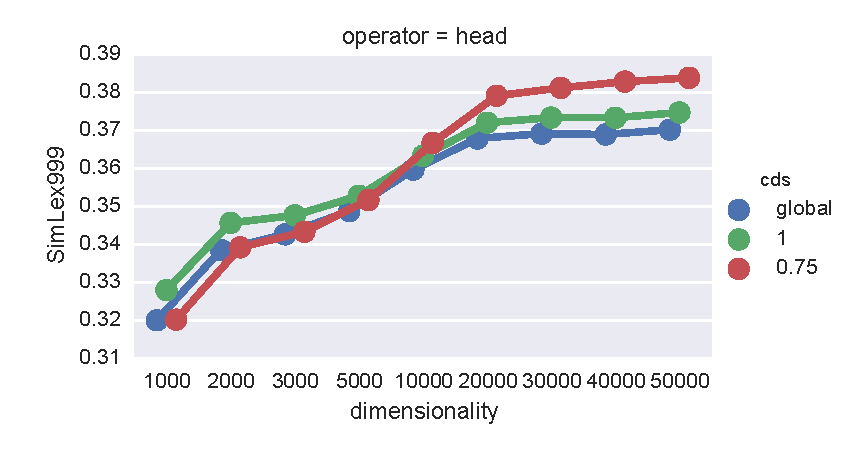
\includegraphics[width=0.5\textwidth]{supplement/figures/SimLex999-interaction-cds}
  \caption{SimLex-999 influence of \texttt{cds}.}
  \label{fig:SimLex999-cds}
\end{wrapfigure}

Finally, models benefit from context distribution smoothing, spaces with less than 10000 dimensions produce the best results with $\alpha = 1$, for spaces with higher dimensionality $\alpha = 0.75$ is the most advantageous (Figure~\ref{fig:SimLex999-cds}). This supports H\ref{hyp:cds} and replicates the results of \newcite{milajevs-sadrzadeh-purver:2016:ACL-SRW}.

\begin{table}
  \centering

  \begin{tabular}{rrlllll}
\toprule
 dimensionality &  SimLex999 &  freq &  discr &   cds &  neg &   similarity \\
\midrule
           1\,000 &      0.328 &  logn &  scpmi &     1 &  0.7 &  correlation \\
           2\,000 &      0.346 &  logn &  scpmi &     1 &  0.7 &  correlation \\
           3\,000 &      0.348 &  logn &  scpmi &     1 &  0.7 &  correlation \\
           5\,000 &      0.353 &  logn &  scpmi &     1 &  0.7 &  correlation \\
          10\,000 &      0.367 &  logn &  scpmi &  0.75 &  0.7 &  correlation \\
          20\,000 &      0.379 &  logn &  scpmi &  0.75 &  0.7 &  correlation \\
          30\,000 &      0.381 &  logn &  scpmi &  0.75 &  0.7 &  correlation \\
          40\,000 &      0.383 &  logn &  scpmi &  0.75 &  0.7 &  correlation \\
          \textbf{50\,000} &      \textbf{0.384} &  \textbf{logn} &  \textbf{scpmi} &  \textbf{0.75} &  \textbf{0.7} &  \textbf{correlation} \\
\bottomrule
\end{tabular}


  \caption{SimLex-999 selection based on heuristics. The highest value is 0.384.
  The values that are grater than 0.361 are indistinguishable from the highest score.}
  \label{tab:Simlex999-heuristics-selection}
\end{table}


\subsection{Difference between Max selection and heuristics on SimLex-999}

As expected, manual parameter selection is more homogeneous as Table~\ref{tab:Simlex999-heuristics-selection} shows. Both selection models agree on parameters for highly dimensional spaces ($D \geq 2000$), with an exception of similarity: Max selection prefers cosine, while manual prefers correlation based similarity measure. Because of this, manual selection does not pick the best result of the 2000 dimensional model, but at 50000 dimensions a model selected manually scores 0.001 lower: 0.384 versus 0.385 as also seen on Figure~\ref{fig:SimLex999-results}.

The average relative difference between Max selection and heuristics is 0.039, which is within the margin set by H\ref{hyp:10percent}.

\section{MEN}
\label{sec:men}

\subsection{Max selection}
\label{sec:max-selection-men}

\begin{figure}
  \centering

    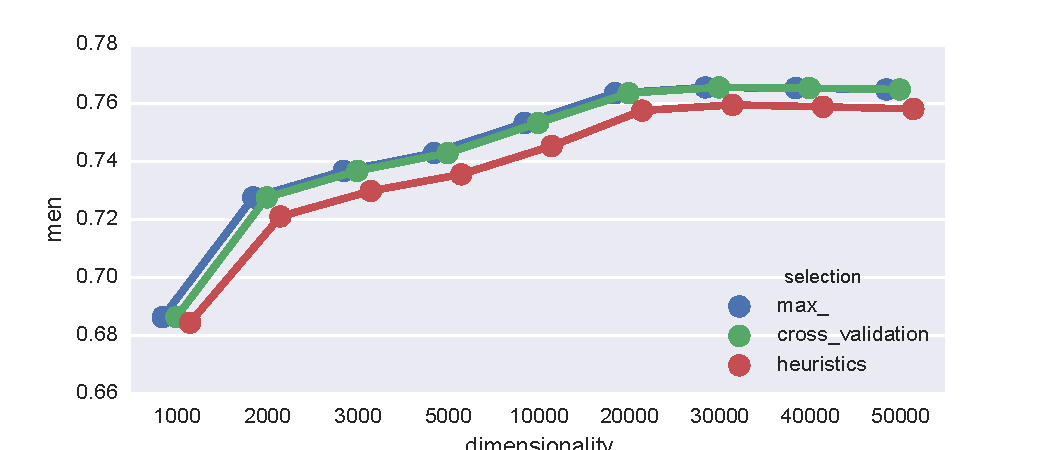
\includegraphics[width=0.5\textwidth]{supplement/figures/men-results}
  \caption{MEN results.}
  \label{fig:men-results}
\end{figure}

%%% Local Variables:
%%% mode: latex
%%% TeX-master: "../thesis"
%%% End:


Figure~\ref{fig:men-results} shows the selection results. Again, cross-validation results are identical with Max selection. Table~\ref{tab:men-max-selection} shows the results together with the selected models.

\begin{table}[b]
  \centering

  \begin{tabular}{rrlllrl}
\toprule
 dimensionality &    men &  freq &  discr &     cds &  neg &   similarity \\
\midrule
           1\,000 &  0.686 &     1 &  scpmi &  global &  1.4 &  correlation \\
           2\,000 &  0.728 &  logn &  scpmi &       1 &  0.7 &          cos \\
           3\,000 &  0.737 &  logn &  scpmi &       1 &  0.7 &          cos \\
           5\,000 &  0.743 &  logn &  scpmi &    0.75 &  0.7 &          cos \\
          10\,000 &  0.753 &  logn &  scpmi &    0.75 &  1.0 &  correlation \\
          20\,000 &  0.763 &  logn &  scpmi &    0.75 &  1.0 &  correlation \\
          \textbf{30\,000} &  \textbf{0.765} &  \textbf{logn} &  \textbf{scpmi} &    \textbf{0.75} &  \textbf{1.0} &  \textbf{correlation} \\
          \textbf{40\,000} &  \textbf{0.765} &  \textbf{logn} &  \textbf{scpmi} &    \textbf{0.75} &  \textbf{1.0} &  \textbf{correlation} \\
          \textbf{50\,000} &  \textbf{0.765} &  \textbf{logn} &  \textbf{scpmi} &    \textbf{0.75} &  \textbf{1.0} &  \textbf{correlation} \\
\bottomrule
\end{tabular}


  \caption{MEN Max selection}
  \label{tab:men-max-selection}
\end{table}


Model performance monotonically increases as the dimensionality increases. The highest score of 0.765 is achieved by 3 spaces with $D \geq 30000$, \logNSCPMI/, smoothed context distribution ($\alpha = 0.75$), shifted PMI values ($k = 1$) and the similarity measure based on correlation.

In comparison with SimLex-999, models with ``more extreme'' parameters give better results. For example, $\alpha = 0.75$ is the best for models tested on SimLex-999 with dimensionality starting with 20000, while for models tested on MEN, this parameter choice is the best starting with 5000. Similar behaviour is observed for \texttt{neg} and similarity. For highly dimensional spaces the switch from SimLex-999 to MEN changes the best \texttt{neg} choice from 0.7 to 1 and similarity from cosine to correlation. Such a switch of parameter choices might suggest the difference between \textit{relatedness} and \textit{similarity}, but it still supports H\ref{hyp:freq}, H\ref{hyp:cds} and H\ref{hyp:neg}.

\subsection{Heuristics}
\label{sec:heuristics-men}

\begin{wraptable}[11]{O}{0.5\textwidth}
  \vspace{1em}
  \centering

  \begin{tabular}{lr}
\toprule
      parameter &  partial $R^2$ \\
\midrule
            neg &  0.309 \\
           freq &  0.204 \\
     similarity &  0.183 \\
          discr &  0.119 \\
 dimensionality &  0.108 \\
            cds &  0.086 \\
\bottomrule
\end{tabular}


  \caption{MEN feature ablation}
  \label{tab:men-ablation}
\end{wraptable}

The linear model gives an adjusted $R^2$ of 0.733, which is lower than on SimLex-999, but is still high. Table~\ref{tab:men-ablation} shows partial $R^2$ scores for the explored parameters. The most influential parameter is \texttt{neg}, followed by \texttt{freq} and similarity. This is different in case of SimLex-999 where these parameters influence ``order'' is reversed.

\begin{figure}
% \begin{wrapfigure}{O}{0.5\textwidth}
  % \vspace{-30pt}
  \centering

  \begin{subfigure}[t]{0.49\textwidth}
    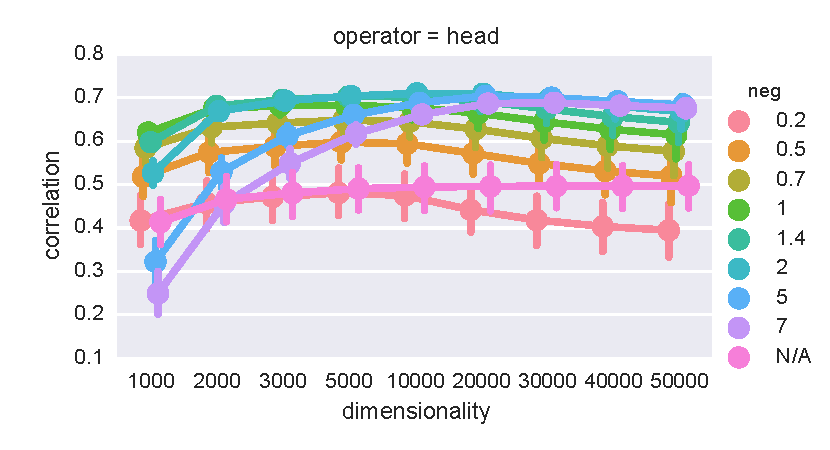
\includegraphics[width=\textwidth]{supplement/figures/men-interaction-neg}

  \caption{\texttt{neg}}
  \label{fig:men-neg}
  \end{subfigure}
  \begin{subfigure}[t]{0.49\textwidth}
    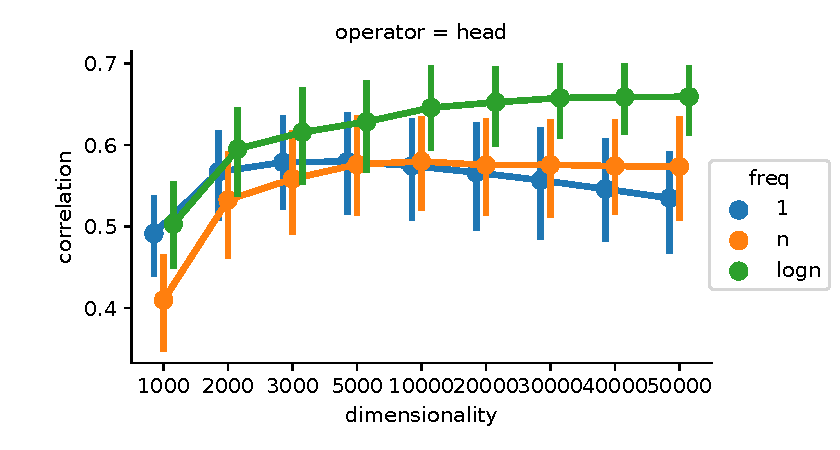
\includegraphics[width=\textwidth]{supplement/figures/men-interaction-freq}

  \caption{\texttt{freq}}
  \label{fig:men-freq}
  \end{subfigure}

  \caption{MEN.}
\end{figure}

\texttt{neg} with $k = 2$ is preferable for spaces with dimensionality less than 20000, for spaces with more dimensions,
$k = 5$ is more beneficial (Figure~\ref{fig:men-neg}). This replicates suggestions of \newcite{TACL570}). We, however, expect that for spaces with more than 500000 dimensions even higher values should be preferred. This contrasts with the heuristics derived from SimLex-999, where single \texttt{neg} value of 0.7 is chosen, but still complies with H\ref{hyp:neg}.

Regarding the frequency component, $\log n$ outperforms all other choices (Figure~\ref{fig:men-freq}). It is exactly the same behaviour as for heuristics based on SimLex-999 including the fact that $1$ and $\log n$ behave similarly for $D \leq 50000$, so H\ref{hyp:freq} is once again confirmed.

\begin{figure}[b]
% \begin{wrapfigure}{O}{0.5\textwidth}
  % \vspace{-30pt}
  \centering
  \begin{subfigure}[t]{0.49\textwidth}
    \hspace{-20pt}
    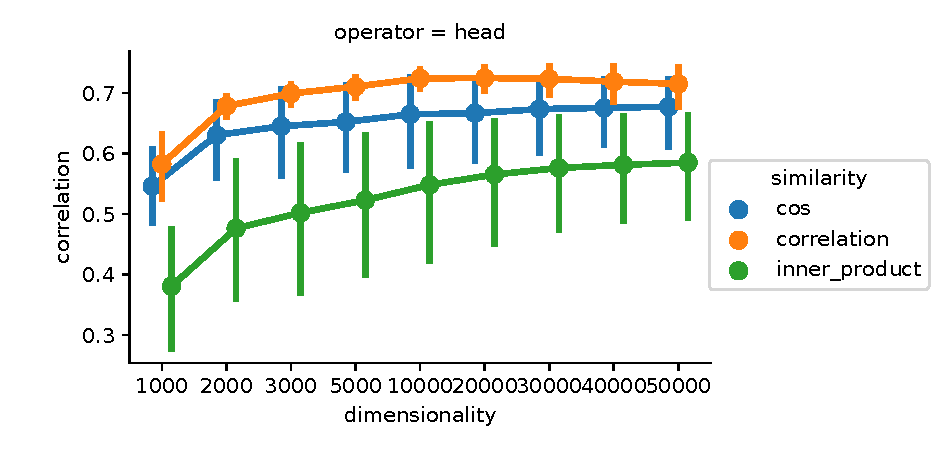
\includegraphics[width=1.1\textwidth]{supplement/figures/men-interaction-similarity}

  \caption{MEN influence of similarity.}
  \label{fig:men-similarity}
  \end{subfigure}
  \begin{subfigure}[t]{0.49\textwidth}
    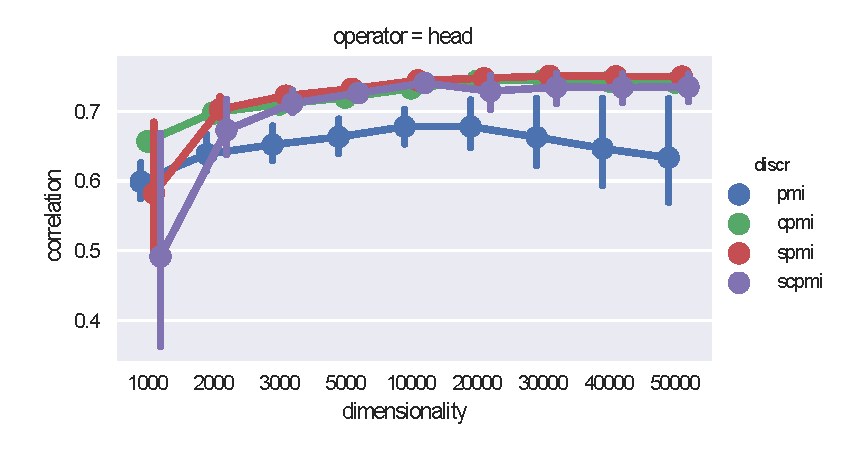
\includegraphics[width=\textwidth]{supplement/figures/men-interaction-discr}

  \caption{MEN influence of \texttt{discr}.}
  \label{fig:men-discr}
  \end{subfigure}
\end{figure}

Correlation is the preferred similarity measure (Figure~\ref{fig:men-similarity}), again this is inline with the choice based on SimLex-999.

SPMI is the preferred discriminativeness (Figure~\ref{fig:men-discr}), however it is closely followed by CPMI and SCPMI. This contrasts with SimLex-999, where SCPMI is preferred, however in both cases the difference between the two discriminativeness choices is minimal. This is inline with H\ref{hyp:lex-pmi-cpmi}.

\begin{figure}
%\begin{wrapfigure}[9]{O}{0.5\textwidth}
  % \vspace{-30pt}
  \centering

  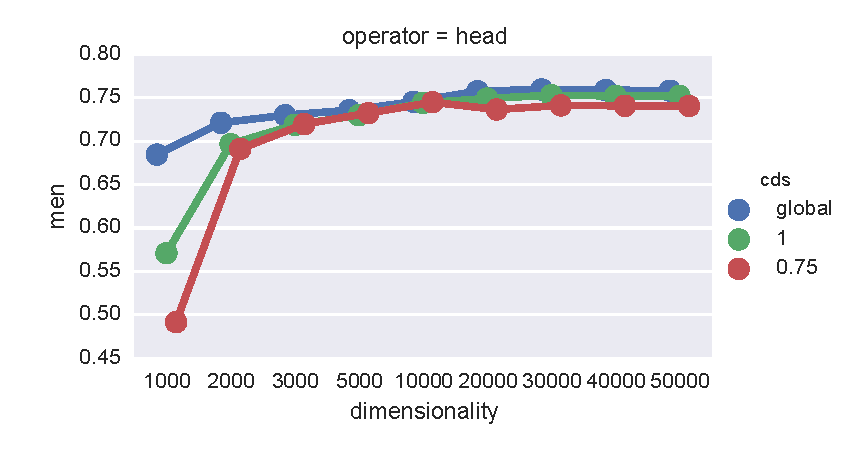
\includegraphics[width=0.5\textwidth]{supplement/figures/men-interaction-cds}

  \caption{MEN influence of \texttt{cds}}
  \label{fig:men-cds}
\end{figure}

Global context probability gives on average higher results for MEN (Figure~\ref{fig:men-cds}). Note, SimLex-999 prefers context distribution smoothing (Figure~\ref{fig:SimLex999-cds}). The difference in performance between local context probabilities and global context probabilities decreases as dimensionality increases, making a weak support of H\ref{hyp:cds}.

\subsection{Difference between Max selection and heuristics on MEN}

\begin{table}
  \centering

  \begin{tabular}{rrlllll}
\toprule
 dimensionality &    men &  freq & discr &     cds & neg &   similarity \\
\midrule
           1\,000 &  0.684 &  logn &  spmi &  global &   2 &  correlation \\
           2\,000 &  0.721 &  logn &  spmi &  global &   2 &  correlation \\
           3\,000 &  0.730 &  logn &  spmi &  global &   2 &  correlation \\
           5\,000 &  0.735 &  logn &  spmi &  global &   2 &  correlation \\
          10\,000 &  0.745 &  logn &  spmi &  global &   2 &  correlation \\
          20\,000 &  0.757 &  logn &  spmi &  global &   5 &  correlation \\
          \textbf{30\,000} &  \textbf{0.759} &  \textbf{logn} &  \textbf{spmi} &  \textbf{global} &   \textbf{5} &  \textbf{correlation} \\
          \textbf{40\,000} &  \textbf{0.759} &  \textbf{logn} &  \textbf{spmi} &  \textbf{global} &   \textbf{5} &  \textbf{correlation} \\
          50\,000 &  0.758 &  logn &  spmi &  global &   5 &  correlation \\
\bottomrule
\end{tabular}


  \caption{MEN selection based on heuristics. The highest value is 0.759. The
    values that are greater than 0.746 are indistinguishable from the highest score.}
  \label{tab:men-heuristics-selection}
\end{table}


The two selection procedures agree on fewer parameters than the ones bases on SimLex-999. Both agree on discrimination ($\log n$) and similarity score for spaces with dimensionality greater than 10000 (correlation). While SCPMI is chosen by Max selection, SPMI is preferred by the selection based on heuristics, however the difference between the two is minimal. In contrast to the Max selection, which chooses the models with context distribution smoothing, heuristics prefer models with global context probabilities. Also, heuristics pick models with higher shifting values $\alpha$ (2 and 5), in contrast to Max selection, where 0.7 and 1 are picked. Table~\ref{tab:men-heuristics-selection} summarises the parameter selection based on heuristics.

The average difference between Max selection and heuristics is 0.008, supporting H\ref{hyp:10percent}.

\section{Selected model transfer to another dataset}
\label{sec:select-model-transf}

\subsection{Difference between heuristics based on MEN and SimLex-999}

Heuristics based on MEN agree with ones bases on SimLex-999 on two parameters: frequency ($\log n$) and similarity (correlation). The methods disagree on \texttt{discr} (SCPMI versus SPMI, but the difference is neglectable as we expect by H\ref{hyp:lex-pmi-cpmi}), context distribution (smoothed versus global) and shifting parameter, for which higher values for MEN are preferred.

\subsection{From SimLex-999 to MEN}

\begin{figure}
  \centering

  \begin{subfigure}[t]{0.49\textwidth}
    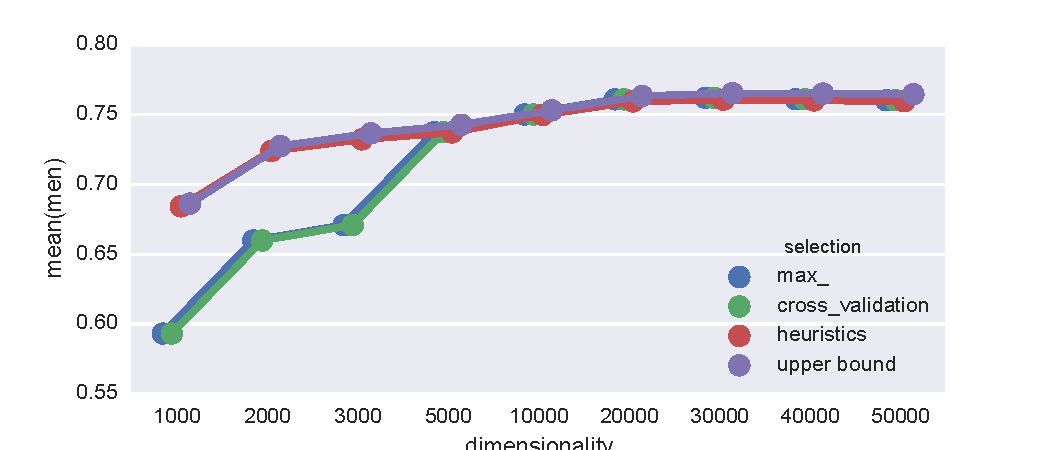
\includegraphics[width=\textwidth]{supplement/figures/SimLex999-transfer}
    \caption{Transfer from SimLex-999 to MEN}
    \label{fig:SimLex999-transfer}
  \end{subfigure}
  \begin{subfigure}[t]{0.49\textwidth}
    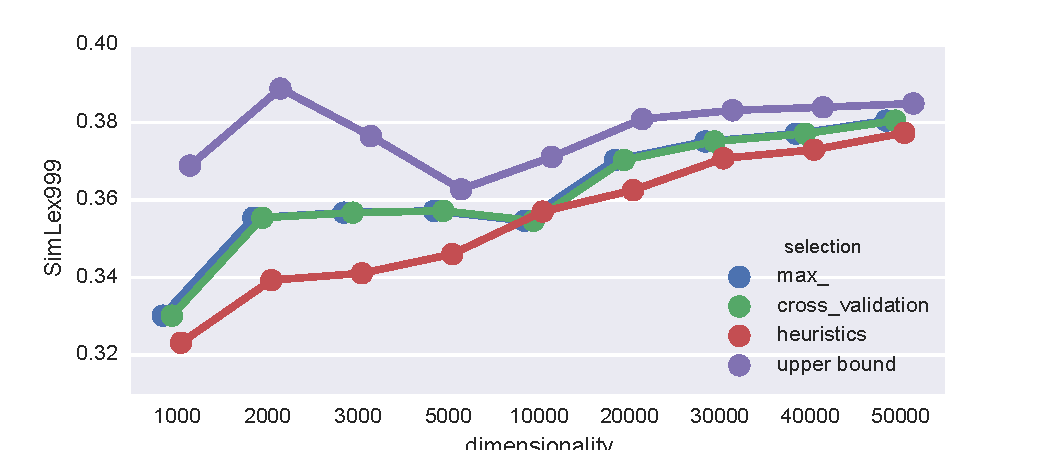
\includegraphics[width=\textwidth]{supplement/figures/men-transfer}
    \caption{Transfer from MEN to SimLex-999}
    \label{fig:men-transfer}
  \end{subfigure}

  \caption{Model transfer between lexical evaluation datasets}
  \label{fig:lexical-transfer}
\end{figure}

%%% Local Variables:
%%% mode: latex
%%% TeX-master: "../thesis"
%%% End:


The models selected using heuristics based on the SimLex-999 dataset perform well on MEN: for all dimensions the selected models are close to the best possible score (Figure~\ref{fig:SimLex999-transfer}). The average difference with the upper bound is 0.006, supporting H\ref{hyp:10percent}.

The max based selection comes close to the upper bound for models with dimensionality greater than 5000. The average difference with the upper bound is 0.039.

In this case, heuristic based selection leads to better performance than the Max based selection, supporting H\ref{hyp:overfitting}.

\subsection{From MEN to SimLex-999}

Heuristics transferred from MEN to SimLex-999 behave less efficient, they do not always outperform Max selection, though for highly dimensional spaces the difference decreases (Figure~\ref{fig:men-transfer}). The average difference is 0.062, which is ten times more than the transition from SimLex-999 to MEN, but still is within the limit set by H\ref{hyp:10percent}.

Max selection neither picks the best possible results when transferred from MEN to SimLex-999, however the average difference is lower: it is 0.042. This is similar to the transition in other direction.

Max based selection leads to better performance than the heuristics for MEN, making a case against H\ref{hyp:overfitting}.

\section{Universal parameter selection for lexical datasets}
\label{sec:universal-lexical-param-selection}

\begin{figure}[b]
  \centering

  \begin{subfigure}[t]{0.49\textwidth}
    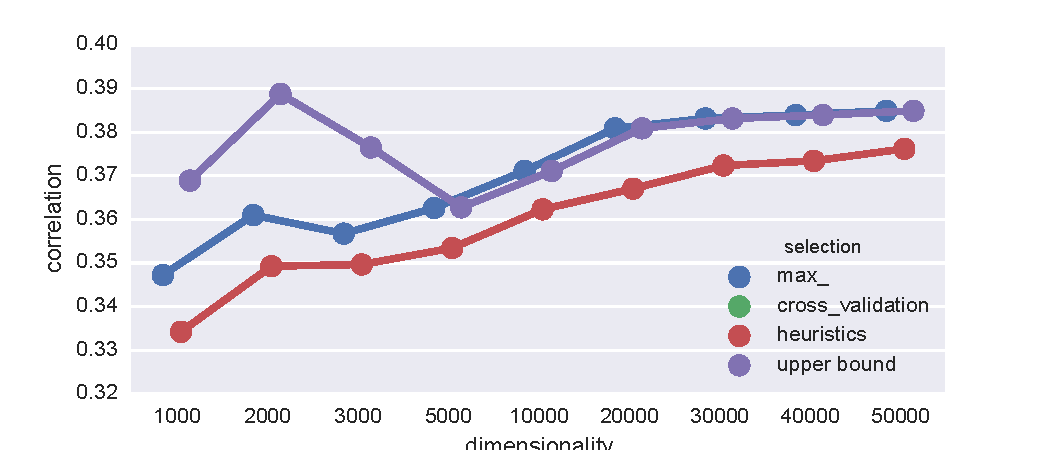
\includegraphics[width=\textwidth]{supplement/figures/lexical-results-SimLex999}
    \caption{SimLex-999}
    \label{fig:lexical-results-simlex}
  \end{subfigure}
  \begin{subfigure}[t]{0.49\textwidth}
    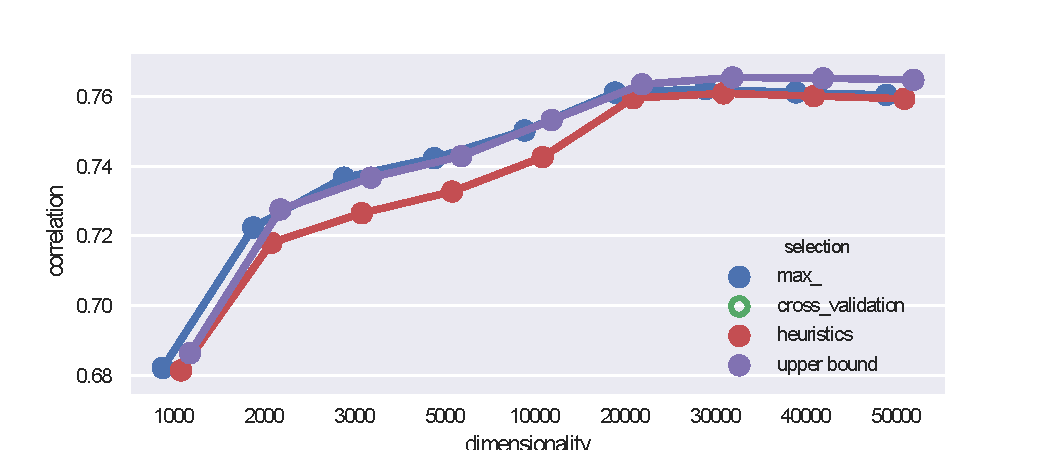
\includegraphics[width=\textwidth]{supplement/figures/lexical-results-men}
    \caption{MEN}
    \label{fig:lexical-results-men}
  \end{subfigure}

  \caption{Performance of models based on the selection over the average lexical performance}
  \label{fig:lexical-results}
\end{figure}

%%% Local Variables:
%%% mode: latex
%%% TeX-master: "../thesis"
%%% End:


Figure~\ref{fig:lexical-results} shows performance of the models based on the average of the normalised scores over SimLex-999 and MEN:
$$
\operatorname{score}_\mathit{lexical}(\mathit{model}) =%
\frac{1}{2}%
\frac{\operatorname{score}_\mathit{SimLex-999}(\mathit{model})}%
{\max_m\operatorname{score}_\mathit{SimLex-999}(m)}%
+%
\frac{1}{2}%
\frac{\operatorname{score}_\mathit{MEN}(\mathit{model})}%
{\max_m\operatorname{score}_\mathit{MEN}(m)}%
$$

The performance of the selected models on both datasets and the normalised average is shown on Table~\ref{tab:lexical-max-selection} (Max selection) and Table~\ref{tab:lexical-heuristics-selection} (selection based on heuristics).

\subsection{Max selection}
\label{sec:max-selection}

In general, the more dimensions, the better the results are. The selection yields the best results at $D = 50000$ for SimLex-999 and at $D = 3000$ for MEN. While for SimLex-999,  the Max selection approaches the upper limit after 20000 dimensions; for MEN, it peaks and slightly deviates from the upper bound as the dimensionality increases.

The Max selection based on the combination of the two lexical datasets is closer to the Max selection based on SimLex-999 (Table~\ref{tab:Simlex999-max-selection}) than on MEN (Table~\ref{tab:men-max-selection}).

\begin{table}
  \centering

  \begin{tabular}{rrrrlllrl}
\toprule
 dimensionality &  SimLex999 &    men &  lexical &  freq &  discr &     cds &  neg & similarity \\
\midrule
           1\,000 &      0.347 &  0.682 &    0.892 &     1 &   spmi &  global &  1.4 &        cos \\
           2\,000 &      0.361 &  0.722 &    0.936 &  logn &  scpmi &  global &  1.0 &        cos \\
           3\,000 &      0.357 &  0.737 &    0.940 &  logn &  scpmi &       1 &  0.7 &        cos \\
           5\,000 &      \textbf{0.363} &  0.742 &    0.951 &  logn &  scpmi &       1 &  0.7 &        cos \\
          10\,000 &      \textbf{0.371} &  \textbf{0.750} &    0.967 &  logn &  scpmi &       1 &  0.7 &        cos \\
          20\,000 &      \textbf{0.381} &  \textbf{0.761} &    0.987 &  logn &  scpmi &    0.75 &  0.7 &        cos \\
          30\,000 &      \textbf{0.383} &  \textbe{0.762} &    0.991 &  logn &  scpmi &    0.75 &  0.7 &        cos \\
          40\,000 &      \textbf{0.384}  &  \textbf{0.761} &    0.991 &  logn &  scpmi &    0.75 &  0.7 &        cos \\
          50\,000 &     \textbe{ 0.385} &  \textbf{0.760} &    \textbe{0.992} &  logn &  scpmi &    0.75 &  0.7 &        cos \\
\bottomrule
\end{tabular}


  \caption[Lexical (combined SimLex-999 and MEN) Max selection]{Lexical (combined SimLex-999 and MEN) Max selection. For the
    individual dataset scores, the scores in bold are indistinguishable from the
  highest score. For SimLex-999, the highest score is 0.385 and the scores above
0.362 are indistinguishable. For MEN, the highest score is 0.762 and the scores
above 0.749 are indistinguishable. The highest combined score is 0.992 and the scores above 0.954 are indistinguishable.}
  \label{tab:lexical-max-selection}
\end{table}


\subsection{Heuristics}

\begin{wraptable}[13]{O}{0.5\textwidth}
  \vspace{3em}
  \centering

  \begin{tabular}{lr}
\toprule
      parameter &  partial $R^2$ \\
\midrule
     similarity &    0.299 \\
            neg &    0.280 \\
           freq &    0.231 \\
 dimensionality &    0.095 \\
          discr &    0.095 \\
            cds &    0.076 \\
\bottomrule
\end{tabular}


  \caption{Lexical feature ablation}
  \label{tab:lexical-ablation}
\end{wraptable}


The linear model achieves an adjusted $R^2$ of 0.817, which is less then $R^2 = 0.867$ of SimLex-999, but is greater than the $R^2 = 0.733$ of MEN. Table~\ref{tab:lexical-ablation} shows partial $R^2$ for each parameter, the most influential are similarity, \texttt{neg} and \texttt{freq}.

\begin{figure}[b]
% \begin{wrapfigure}{O}{0.5\textwidth}
  % \vspace{-30pt}
  \centering

  \begin{subfigure}[t]{0.49\textwidth}
    \hspace{-20pt}
    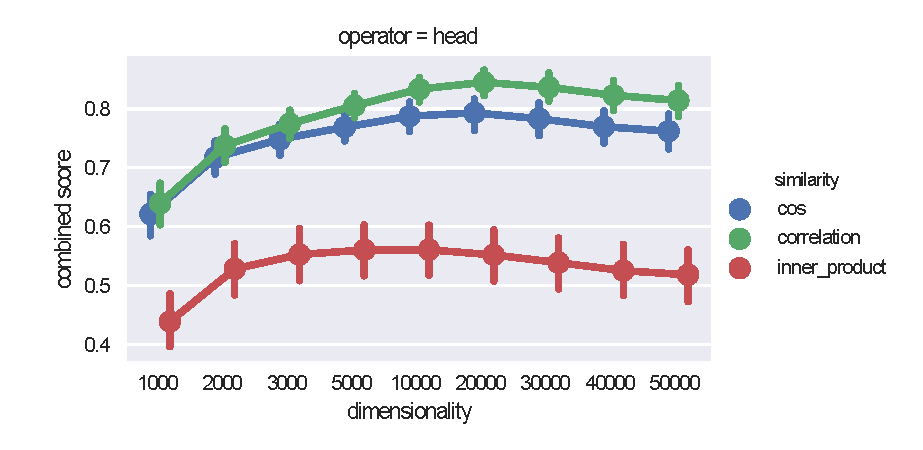
\includegraphics[width=1.1\textwidth]{supplement/figures/lexical-interaction-similarity}

    \caption{Similarity}
    \label{fig:lexical-similarity}
  \end{subfigure}
  \begin{subfigure}[t]{0.49\textwidth}
    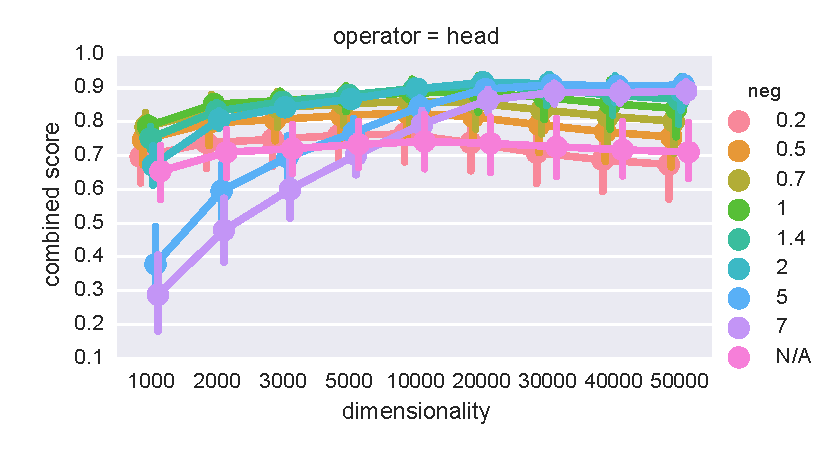
\includegraphics[width=\textwidth]{supplement/figures/lexical-interaction-neg}

    \caption{\texttt{neg}}
    \label{fig:lexical-neg}
  \end{subfigure}
  \caption{Lexical the influence of similarity and \texttt{neg}}
\end{figure}

Correlation is the similarity measure of choice (Figure~\ref{fig:lexical-similarity}). However, the difference between cosine and correlation is minimal for $D \leq 5000$.

For the models with dimensionality less than 20000 shifting should be used with $k = 1$, otherwise $k = 2$ is preferred (Figure~\ref{fig:lexical-neg}). This supports H\ref{hyp:neg}.

\begin{figure}[h]
% \begin{wrapfigure}{O}{0.5\textwidth}
  % \vspace{-30pt}
  \centering

  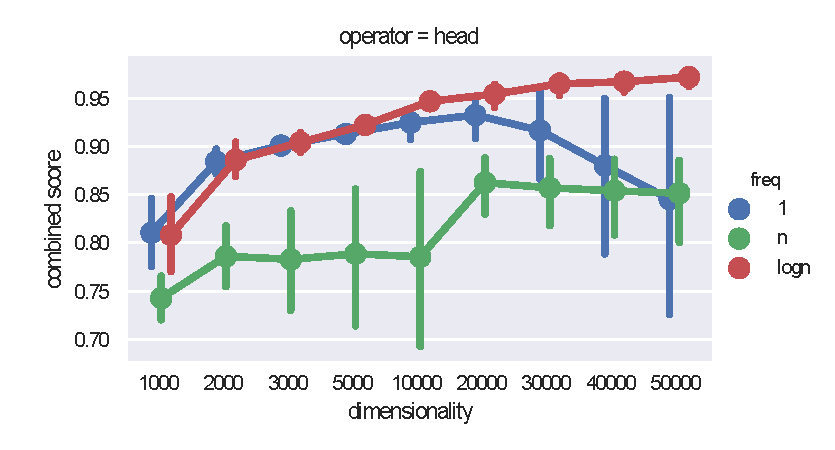
\includegraphics[width=0.5\textwidth]{supplement/figures/lexical-interaction-freq}

  \caption{Lexical influence of \texttt{freq}.}
  \label{fig:lexical-freq}
\end{figure}

$\log n$ on average performs the best as the frequency component (Figure~\ref{fig:lexical-freq}). But for $D \leq 5000$, 1 is also performs competitively to $\log n$, supporting H\ref{hyp:freq}.

SCPMI is the preferred discrimination component, but SPMI is very close to it (Figure~\ref{fig:lexical-discr}) backing up H\ref{hyp:lex-pmi-cpmi}.

% \begin{figure}[h]
\begin{wrapfigure}[7]{O}{0.5\textwidth}
  \vspace{-30pt}
  \centering

  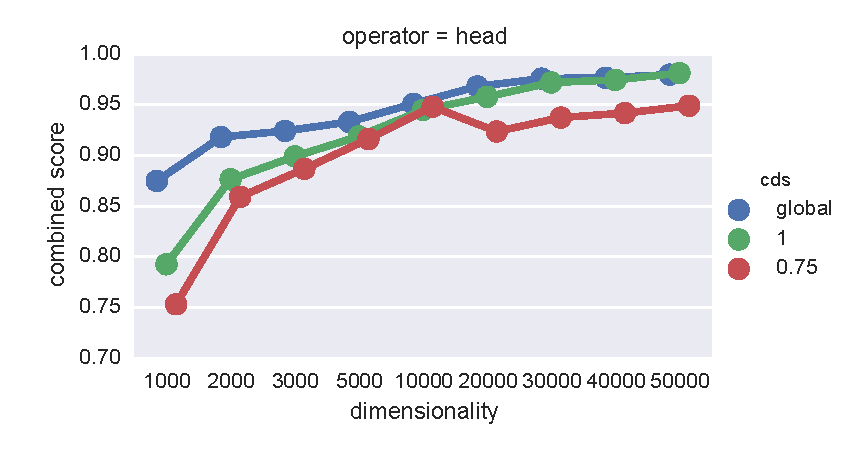
\includegraphics[width=0.5\textwidth]{supplement/figures/lexical-interaction-cds}

  \caption{Lexical influence of \texttt{cds}.}
  \label{fig:lexical-cds}
\end{wrapfigure}

Global context probabilities on average behave the best (Figure~\ref{fig:lexical-cds}). However, global context probabilities and local context probabilities with $\alpha = 1$ yield close results for $D > 10000$, giving support to H\ref{hyp:cds}.

\begin{table}
  \centering

  \begin{tabular}{rrrrlllll}
\toprule
 dimensionality &  SimLex999 &   men &  lexical &  freq &  discr &     cds & neg &   similarity \\
\midrule
           1\,000 &       0.33 &  0.68 &     0.87 &  logn &  scpmi &  global &   1 &  correlation \\
           2\,000 &       0.35 &  0.72 &     0.92 &  logn &  scpmi &  global &   1 &  correlation \\
           3\,000 &       0.35 &  0.73 &     0.92 &  logn &  scpmi &  global &   1 &  correlation \\
           5\,000 &       0.35 &  0.73 &     0.93 &  logn &  scpmi &  global &   1 &  correlation \\
          10\,000 &       0.36 &  0.74 &     0.95 &  logn &  scpmi &  global &   1 &  correlation \\
          20\,000 &       0.37 &  \textbf{0.76} &     0.97 &  logn &  scpmi &  global &   2 &  correlation \\
          30\,000 &       0.37 &  \textbf{0.76} &     \textbf{0.98} &  logn &  scpmi &  global &   2 &  correlation \\
          40\,000 &       0.37 &  \textbf{0.76} &     \textbf{0.98} &  logn &  scpmi &  global &   2 &  correlation \\
          50\,000 &       \textbf{0.38} &  \textbf{0.76} &     \textbf{0.98} &  logn &  scpmi &  global &   2 &  correlation \\
\bottomrule
\end{tabular}


  \caption{Lexical (combined SimLex-999 and MEN) selection based on heuristics.}
  \label{tab:lexical-heuristics-selection}
\end{table}


\subsection{Comparison with single dataset based selections}

Both selection methods mostly agree on frequency ($\log n$) and discriminativeness (SCPMI).

Context probability distribution smoothing varies between the selection methods, but follows the corresponding procedures based on MEN.

The Max based selection for \texttt{neg} follows the Max selection on SimLex-999.

Even though the similarity choice is different between the Max and heuristic selections, it is consistent with SimLex-999 in both cases and with MEN for the heuristic-based selection.

For the Max-based selection, the average difference is 0.020 on SimLex-999 and 0.004 for MEN.

For the heuristics-based selection, the average difference is 0.048 for SimLex-999 and 0.010 for MEN, which is within the 10\% limit set by H\ref{hyp:10percent}.

Max selection behaves better than the heuristics based on the average difference, but we can not check how well these two selections behave on other lexical datasets. This is an evidence against H\ref{hyp:overfitting}.

Based on the experiments, \logNSCPMI/ with shifting close to 1 is the quantification of choice for the lexical tasks, however more work needs to be done to find robust choice for context distribution smoothing and similarity measure.

\section{Conclusion}
\label{sec:conclusion-lexical}

Lexical experiments give support to the most of the stated hypotheses in Sections~\ref{sec:hypotheses} and \ref{sec:elab-hypoth-lexical}.

The optimal parameter choice depends on dimensionality (H\ref{hyp:dimen}). In particular, non constant frequency component (Section~\ref{sec:frequency-weighting}), H\ref{hyp:freq}), context distribution smoothing (Section~\ref{sec:cont-distr-smooth}, H\ref{hyp:cds}) and shifting (Section~\ref{sec:shifted-pmi}, H\ref{hyp:neg}) should be applied for spaces with $D \geq 10000$.

The switch at 10000 dimensions is a ``parameter sweet spot'' as parameter choice is not significant at these points, the most representative example is the behaviour of \texttt{cds} on SimLex-999 (Figure~\ref{fig:SimLex999-cds}. After that point performance either converges (supporting H\ref{hyp:var}), as in case of \texttt{neg} on SimLex-999 (Figure~\ref{fig:SimLex999-neg}), or there is one dominant choice, as for \texttt{freq} on SimLex-999 (Figure~\ref{fig:SimLex999-freq}).

As expected, we did not see a significant influence of the ``compression'' of the PMI values (H\ref{hyp:lex-pmi-cpmi}).

We could not find supporting evidence for H\ref{hyp:overfitting}, as Max-selected models performed well on transfer and both selection methods are within the 10\% difference margin to the highest result (H\ref{hyp:10percent}), suggesting that there indeed might be a universal vector space (H\ref{hyp:universal}).

We observed another regularity: cosine is a good similarity choice for low-dimensional spaces, but correlation is a better choice for highly-dimensional spaces.

%%% Local Variables:
%%% mode: latex
%%% TeX-master: "thesis"
%%% End:
